% !TeX encoding = UTF-8
% !TeX root = ../thuthesis-example.tex

\chapter{引言}
\label{ch1}
\section{研究背景及意义}
人工智能(Artificial Intelligence)在过去十几年来的蓬勃发展让现实生活中的许多领域变得日趋无人化与智能化:增强现实(AR)使人能够和虚拟环境进行互动;自动驾驶技术(self-driving technology)的落地与应用使得道路更加智能化,提升了道路运输的安全性与便利性\cite{paden2016survey};智能机器人的发明,一方面如扫地机器人的出现使得智能家居领域得到发展;另一方面在工业领域移动机器人的出现使得人们从重复性高或危险性高的工作当中得以解放\cite{cheng2005study}。图\ref{application}列举了常见的几种智能化领域。
\begin{figure}
	\centering
	\subcaptionbox{增强现实}
	{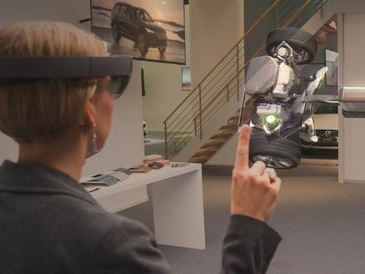
\includegraphics[width=5.5cm]{vr}}
	\subcaptionbox{自动驾驶}
	{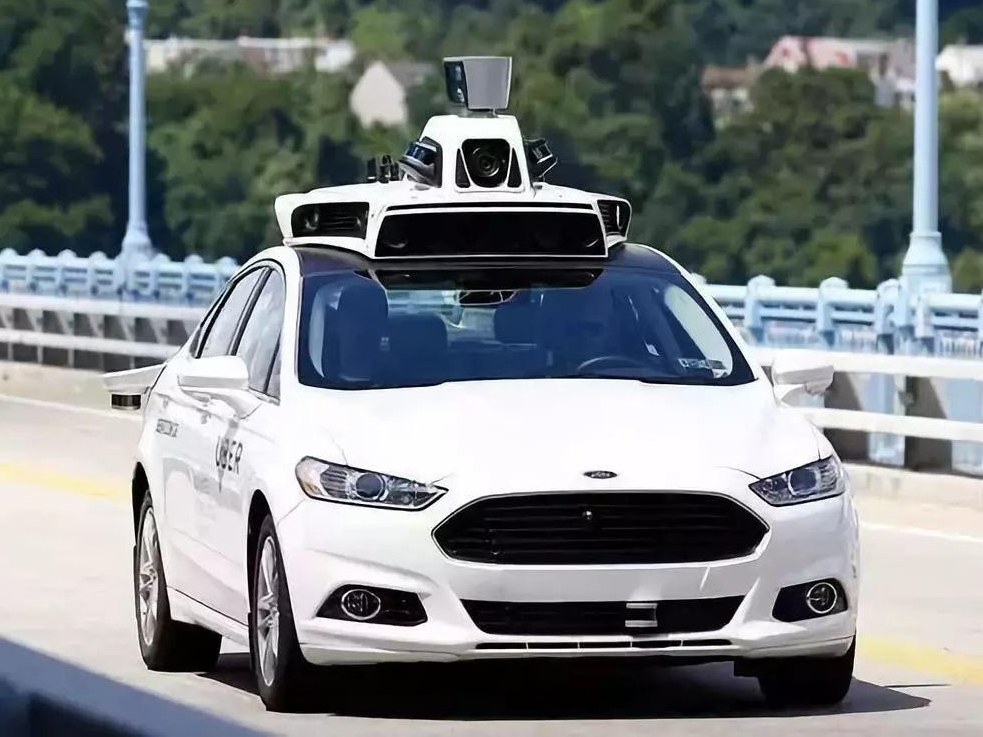
\includegraphics[width=5.5cm]{auto-car}}\\
	\subcaptionbox{扫地机器人}
	{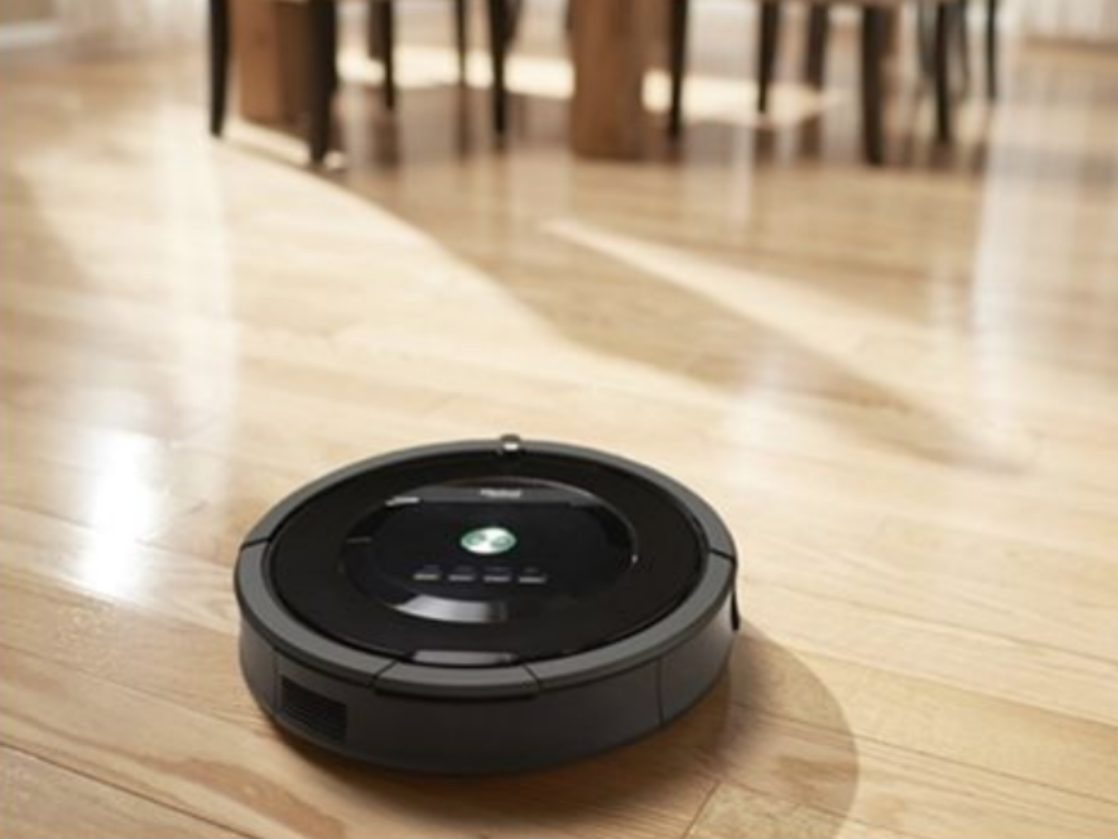
\includegraphics[width=5.5cm]{sweep-robot}}
	\subcaptionbox{移动机器人}
	{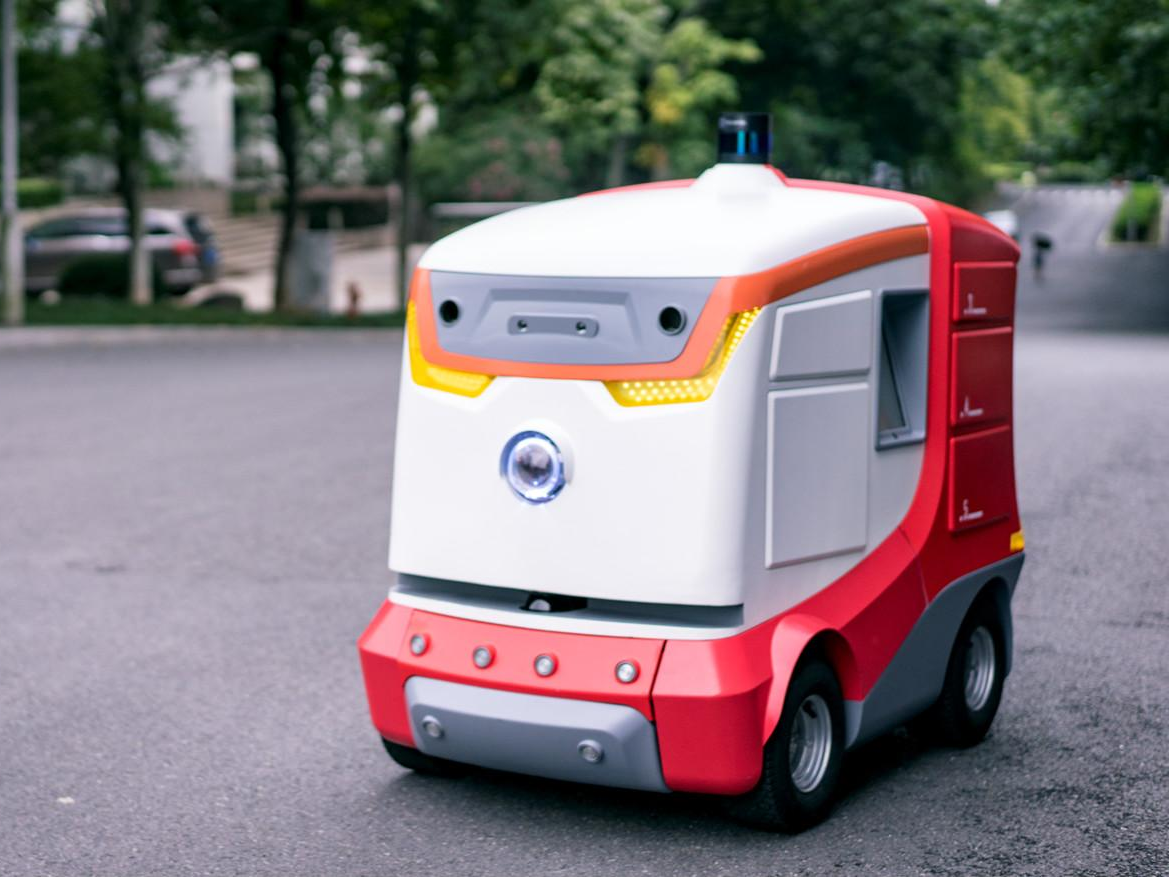
\includegraphics[width=5.5cm]{move-robot}}
	\caption{近年常见智能化领域}
	\label{application}
\end{figure}

以上几种智能化技术的应用,离不开对于场景的构建与定位工作。场景构建是指对一个真实的环境采用特定的模型进行数学描述,在计算机视觉领域,一般通过构建场景的点云模型来进行建模,一个准确、高精度的场景点云模型能够为定位系统提供更好的基础。定位是指移动机器人通过自身的传感器获取数据,对外界环境信息进行感知与处理,通过图像处理技术或点云处理技术来计算移动机器人的位置。定位任务又可以分成两个部分:绝对定位与相对定位。绝对定位是指计算自身在环境中的绝对位置,而相对定位是指在机器人的运动过程中估计每一时刻与上一时刻的相对运动,从而恢复出整个运动轨迹。

在图\ref{application}的各个领域中,场景构建与定位都发挥着重要作用。在自动驾驶领域,一个准确的定位能够提升无人汽车的安全性;一个高精度地图的构建能够提升用户在增强现实上的体验;同时一个鲁棒且准确的建图定位算法也能够提升工业机器人的工作效率与准确性。

如今,在处理建图与定位任务时主要采取两种方向:

第一,同时建图与定位。这里的定位解决的是相对定位,即机器人在环境中移动的时候,利用环境信息特征,一边推测自己的相对位姿从而恢复轨迹,一边进行地图构建,当机器人完成整体环境的探测时,也完成了地图的构建。同时建图与定位算法被称为SLAM算法(Simultaneous Localization and Mapping)。

第二,先建图后定位。这里的定位指的是绝对定位,不同于SLAM算法,它需要机器人首先对全局环境进行了解,从而将其放入环境中时,能够准确定位出机器人的绝对位置。对于建图任务,常用的方法有基于单目视觉的SfM(Structure-from-Motion)算法,能利用图像稀疏地构建环境三维模型。对于室内定位任务,常采用的方法是提前在场景粘贴视觉marker,并在重建地图中进行标记,以此来进行检测与定位\cite{babinec2014visual, zheng2018visual},常用的视觉marker有Aruco\cite{garrido2014automatic}等;在室外环境中,通常利用GPS信号进行辅助定位\cite{reina2007adaptive}。
\begin{figure}
	\centering
	\subcaptionbox{双目相机\label{double-eye}}
	{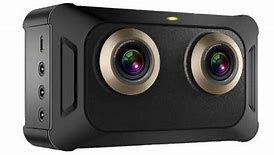
\includegraphics[height=3cm]{double-eye}}
	\subcaptionbox{RGB-D相机\label{realsense}}
	{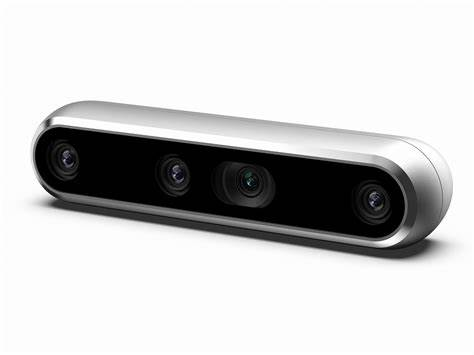
\includegraphics[height=3cm]{realsense}}
	\subcaptionbox{激光雷达\label{livox}}
	{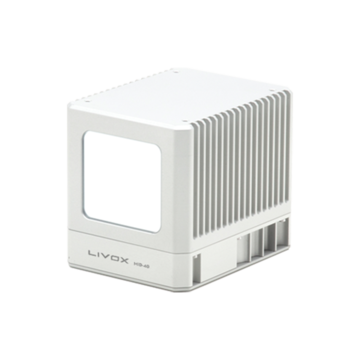
\includegraphics[height=3cm]{livox}}
	\caption{实验设备}
	\label{sensor}
\end{figure}

随着技术的进步,各种传感设备正在不断更新,如图\ref{sensor}所示,双目相机、RGB-D相机、激光雷达的出现使得对于环境数据的采集变得更加便捷、数据类型更加多样。但尽管如此,在重建与定位的算法方面仍面临着不少挑战,主要有如下几点:
\begin{enumerate}
	\item \textbf{大场景的精确重建具有挑战性。}对于大场景的重建问题,通常有两种解决方式,第一种是依靠传统的SLAM或SfM算法进行一次性重建,但在大场景构建中前者会存在尺度模糊与漂移问题\cite{huang2019survey},后者由于搜索数据的增加造成算法效率低下。另一种解决方式是先对局部场景进行构建,再进行融合,这需要一个有效的点云融合算法进行支撑。
	\item \textbf{视觉定位需要具有鲁棒性。}在利用视觉进行定位的算法中,常常面临着不够鲁棒的问题:因为受时间及环境变化的影响,建图与定位时场景中的光照细节可能发生较大的变化,这个容易给传统图像匹配算法的性能造成影响。
	\item \textbf{传感器对定位性能的限制。}采用激光雷达设备,其实时性较差,并且成本较高,不利于长期性、实时性的定位需求,而利用传统的单目相机进行视觉定位,由于视野较窄、视角方向单一,在场景中容易由于受到遮挡,或环境特征不够明显时出现定位丢失的现象。
\end{enumerate}

根据以上挑战,本文提出了一套对于大场景的建图与定位算法。首先它采用了从局部到整体的思路来减少漂移现象,先选择合适的方式构建场景局部点云,然后对不同局部的点云进行有效地融合,完成重建任务。在视觉定位上,选择了全景相机作为传感器设备,能够覆盖比传统相机更广的范围,捕捉比激光雷达更远的视觉信息;并为了克服跨模态图像的差异,采用了基于神经网络的特征匹配方法,提升了定位过程中的鲁棒性。

\section{研究现状}
\subsection{视觉三维重构}
目前基于视觉三维重构主要有两个流行的方向,第一个是采用视觉SLAM的方法,按照一定的采样率对场景进行连续的图像拍摄,并依靠算法在定位的同时恢复场景的整体图像;第二个是采用SfM方法,提前在场景中拍摄大量无序照片,通过搜索匹配的方式发现重叠图像,进而恢复场景模型。本小节分别对于这两种视觉三维重构方法的研究现状进行了总结。

\textbf{1. Simultaneous Localization and Mapping}

SLAM的整体框架如图\ref{slam-structure}所示,其架构包括前端和后端两个部分\cite{cadena2016past}。其中前端利用传感器的数据,估计出传感器的运动,从具体实现上,该模块首先从传感器数据中提取特征,然后寻找特征之间的关联,从而从短期上看可以估计出相邻两帧传感器数据之间的运动,从长期看能够通过判断新特征是否与之前数据中的特征相似来进行回环检测。由于传感器数据存在噪声、特征提取与配对不能做到完全准确,因此在估计运动时不可避免地会出现误差,这一误差会随着传感器的运动而逐渐累积,而SLAM框架中的后端则是通过优化算法,来消除累积误差,从而得到更为准确的地图及运动轨迹。
\begin{figure}
	\centering
	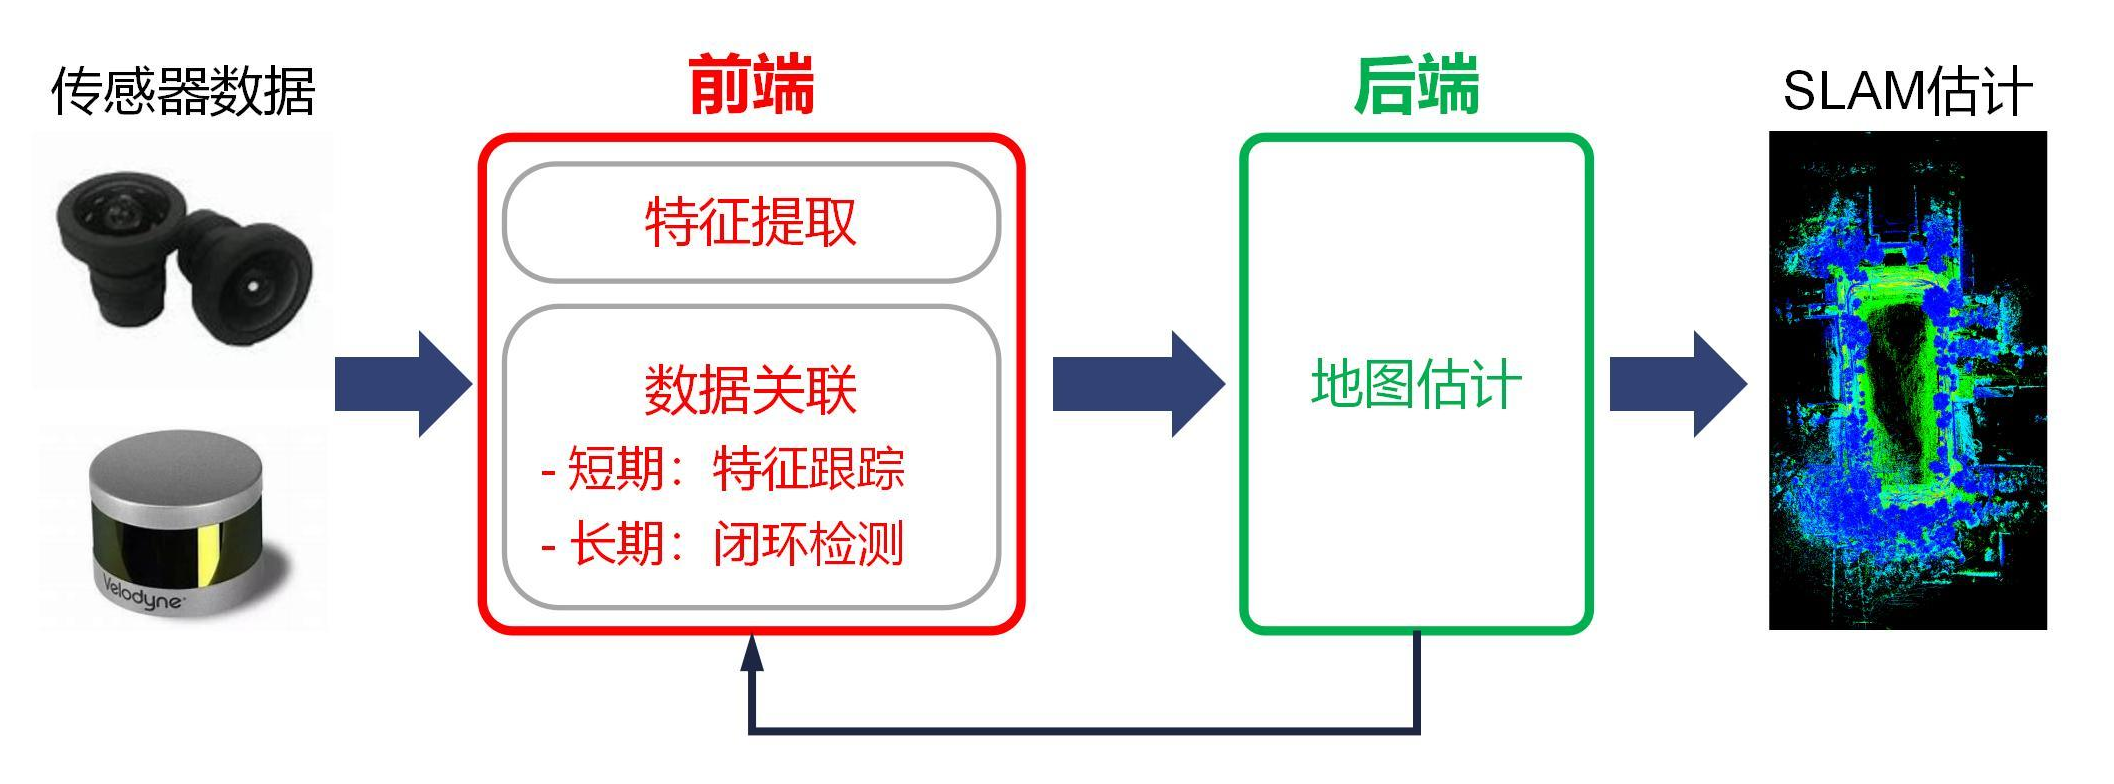
\includegraphics[width=13cm]{slam-structure}
	\caption{典型SLAM系统中的前端与后端}
	\label{slam-structure}
\end{figure}

若上图中的传感器为相机,则相关的SLAM算法则被称为视觉SLAM(VSLAM),即利用图像特征进行建图与定位。本小节以VSLAM为例,介绍几种当前常见的算法及框架。

MonoSLAM是第一个仅利用单目相机进行实时建图与定位的框架\cite{davison2007monoslam}。MonoSLAM能够对图像中的特征点进行提取,并追踪其运动,同时利用扩展卡尔曼滤波器(EKF)的方式对当前状态进行更新,并调整landmark状态的均值和协方差矩阵。根据EKF的原理,特征点的位置服从三维空间中的高斯分布,通过连续观测,能够降低位置的不确定性,从而使定位精度逐渐收敛,这一算法框架适用于小范围的场景,具有较好的实时性。
\begin{figure}
	\centering
	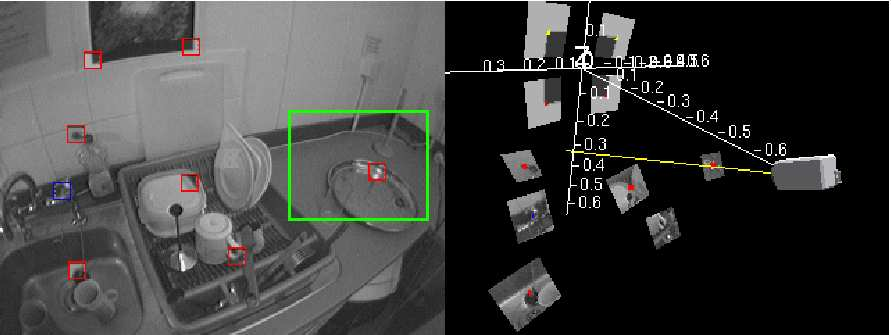
\includegraphics[width=14cm]{monoslam}
	\caption{MonoSLAM特征检测与地标效果图}
	\label{monoslam}
\end{figure}

SLAM技术的第二个里程碑是\citet{klein2007parallel}提出的PTAM。PTAM算法第一次将SLAM任务分解为前端和后端两个部分,这为之后许多VSLAM的系统设计提供了参照。不同于传统算法中以滤波方式进行优化,PTAM算法采用非线性优化作为后端算法。同时为图像序列标记关键帧,避免了对所有图像的冗余处理,提升了轨迹估计和地图重建的速度,保证了算法的实时性。PTAM提出后,有基此算法开发的AR软件问世,能够利用相机对环境中的平面进行感知,从而逼真地在真实环境中展示虚拟物品。
\begin{figure}
	\centering
	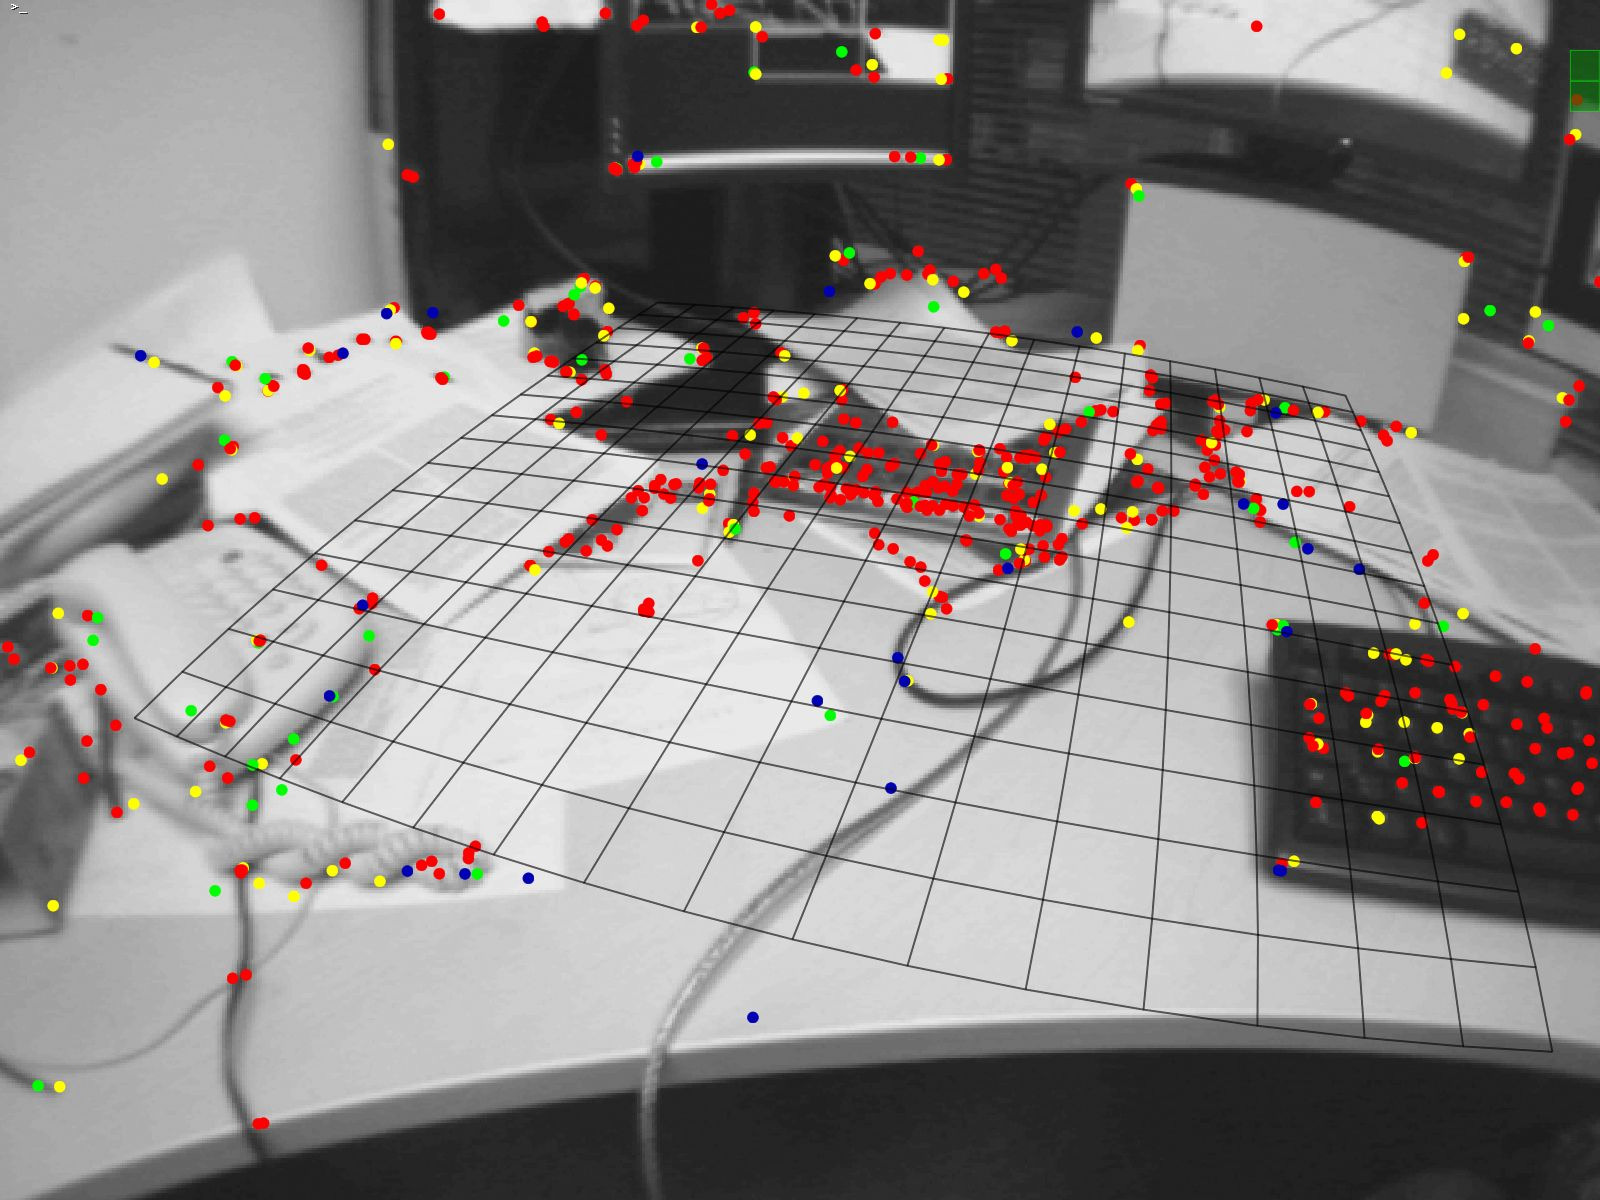
\includegraphics[width=10cm]{ptam}
	\caption{PTAM算法效果图}
	\label{ptam}
\end{figure}

2015年,\citet{mur2015orb}提出了ORB-SLAM,该算法在PTAM的基础上能够自动生成初始化地图,并通过特征比对判断闭环,同时在关键帧选择与特征提取方法上进行了优化,得到了实时性和精度更好的效果。ORB-SLAM的框架如图\ref{orbslam}所示,可以分为跟踪、建图、重定位与闭环检测四大部分。在跟踪阶段,ORB-SLAM采用了ORB描述子\cite{rublee2011orb}对图像特征进行描述,能够更好地提升特征提取的速度,同时具有光照不变性,因此更加鲁棒;在建图模块中,算法通过特征点不断生成新的局部地图点,筛选后插入点云地图中,该部分同时实现了关键帧的筛选以及去除功能;闭环检测模块中,首先对关键帧记性检测判断回环,当回环出现时,使用地图融合技术对地图中重复的点云进行融合,并采用Essential Graph的方式对回环进行优化,使得地图更好地闭合。最终,该算法实现了在不依赖多线程与GPU的情况下,达到了30fps的追踪速度,因此适用于实时SLAM中。在ORB-SLAM的基础上,作者还于2017年发布了基于双目相机与RGB-D相机的ORB-SLAM2算法\cite{mur2017orb}。
\begin{figure}
	\centering
	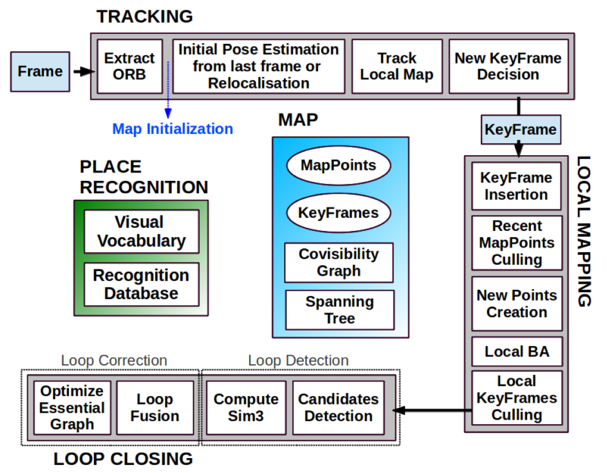
\includegraphics[width=13cm]{orbslam}
	\caption{ORB-SLAM流程图}
	\label{orbslam}
\end{figure}

近年来,得益于深度学习的不断发展与进步,不少学者将其融入到传统的SLAM算法之中。该类算法的思路往往是利用深度学习的方法对SLAM框架中的一个或多个模块进行替换,达到更加鲁棒的效果。

CNN-SLAM\cite{tateno2017cnn}算法利用CNN网络对关键帧图像的深度进行了估计,并与传统SLAM算法中得到的深度进行融合,从而优化特征点的位置,同时也使用神经网络对图像的语义信息进行跟踪,得到了语义连贯的重建结果,CNN-SLAM在低纹理区域等场景中得到了比传统方法更鲁棒和准确的结果。
\begin{figure}
	\centering
	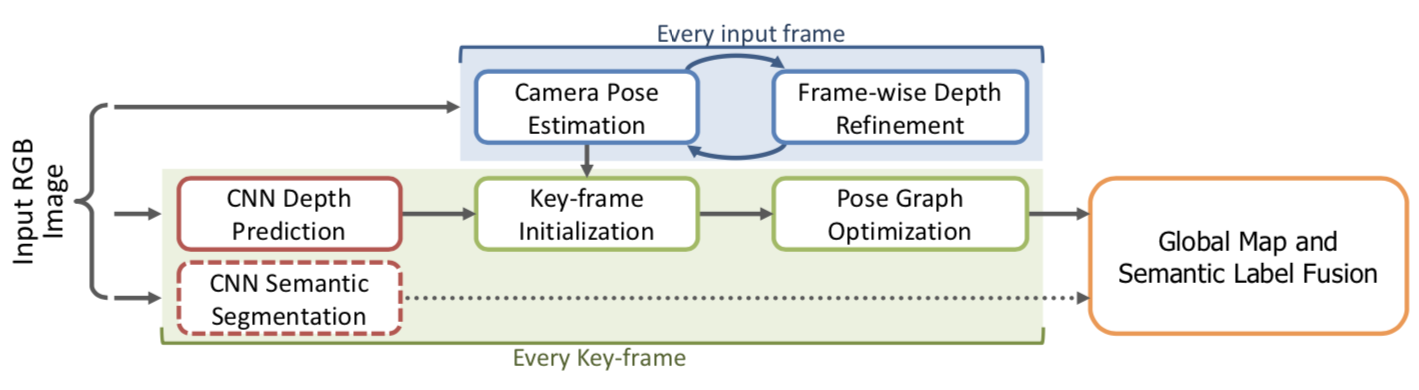
\includegraphics[width=14.5cm]{cnn-slam}
	\caption{CNN-SLAM流程图}
	\label{cnn-slam}
\end{figure}

\citet{detone2017toward}采用深度学习,替换了传统SLAM框架中的特征点提取和匹配模块。首先利用MagicPoint网络对单帧图像的关键点进行提取,相比于传统特征描述子,该网络在图像有噪声的情况下能够更鲁棒地提取到有用的关键点。第二个网络是MagicWarp,它仅以MagicPoint网络输出一系列图像点对的坐标作为输入,在不依赖于局部点描述子的情况下估计$3\times 3$的单应性矩阵,进而恢复相机的转移,该算法同样在单核CPU上实现了30fps的实时SLAM。
\begin{figure}
	\centering
	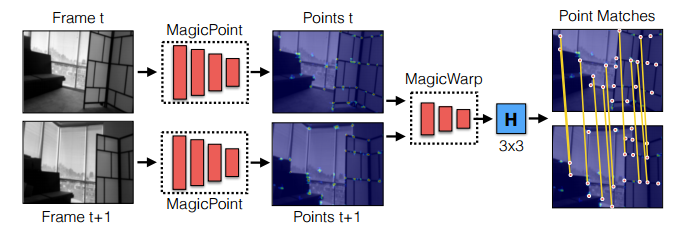
\includegraphics[width=14.5cm]{magic-slam}
	\caption{面向几何的深度SLAM框架}
	\label{magic-slam}
\end{figure}

\textbf{2. Structure-from-Motion}

在SfM方面,来自华盛顿大学的研究人员\citet{snavely2006photo}最早为这一算法提供了流程上的基础。在Photo Tourism项目中,他们从各大照片网站中爬取同一个景点的不同照片,利用SIFT算法\cite{lowe2004distinctive}提取图像中的描述子,然后对图像中的特征点两两进行匹配,利用对应点的几何关系重建出场景模型。利用该算法,他们对意大利罗马的特莱维喷泉和中国的万里长城进行了场景重建,如图\ref{photo-tourism}所示,都证明了这一流程是可行的。
\begin{figure}
	\centering
	\subcaptionbox{特莱维喷泉\label{tourism-fountain}}
	{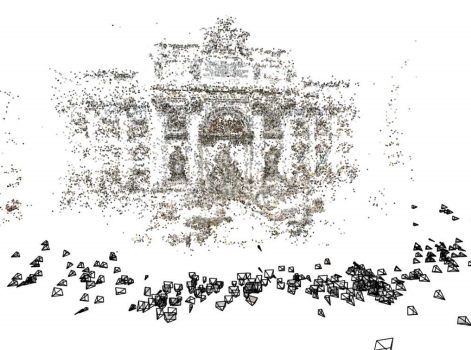
\includegraphics[width=6.5cm]{tourism-fountain}}
	\subcaptionbox{长城\label{tourism-great-wall}}
	{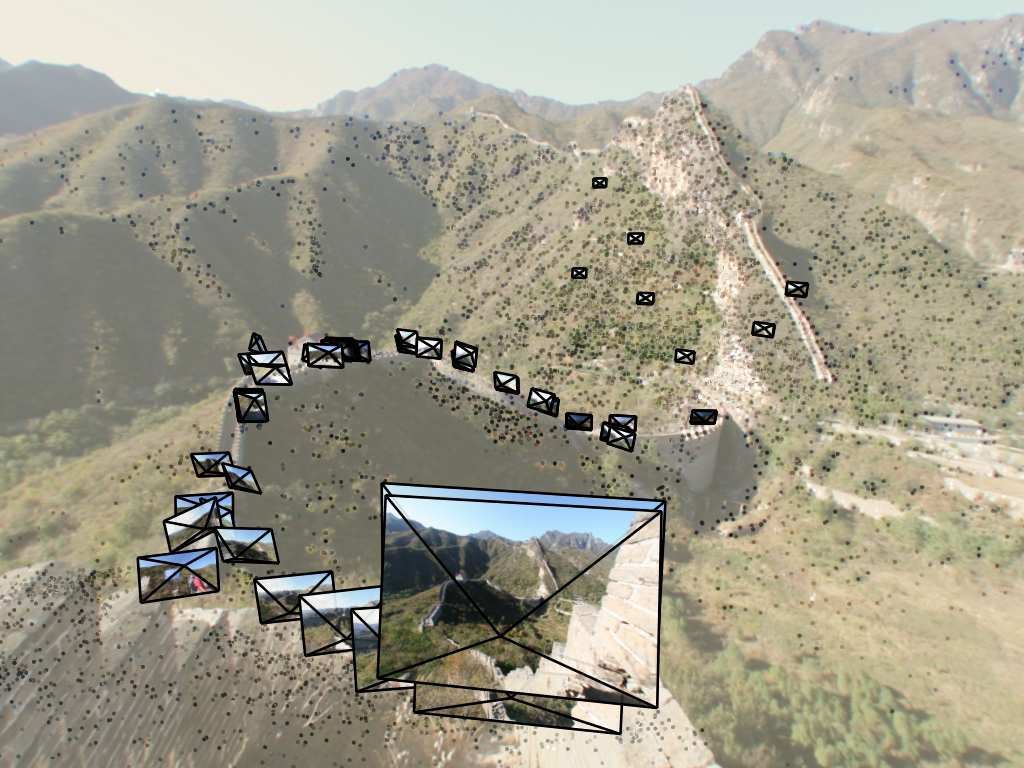
\includegraphics[width=6.5cm]{tourism-great-wall}}
	\caption{Photo Tourism场景重建}
	\label{photo-tourism}
\end{figure}

对于Photo Tourism中的算法,由于其需要进行大量的匹配和搜索,因此复杂度达到了$O(n^4)$,其中$n$为照片的数量。随着VisualSFM算法\cite{wu2011visualsfm}的提出,这一复杂度被下降到$O(n^2)$,同时也对重建的精度得到了较好的保留。得益于SIFT算法在GPU上的运行\cite{acharya2013speeding},该算法的效率更是得到了较大的提升,在此方法发表后,基于VisualSFM算法的GUI应用也被开发了出来,方便了重建的流程。

以上SfM算法均为增量式的重建算法,\citet{moulon2013global}在2013年提出了全局式的SFM算法,相比于增量式的SfM中一边重建一边进行局部优化带来的效率低下、并且容易出现漂移性的问题,全局式的SfM算法先对所有图像计算关键点,利用对应关系求取变换,最后通过一次性的优化对整体进行调整,这大大提高了算法效率,但该算法容易受到一些噪声图像的影响,因此相对而言鲁棒性较差。
\begin{figure}
	\centering
	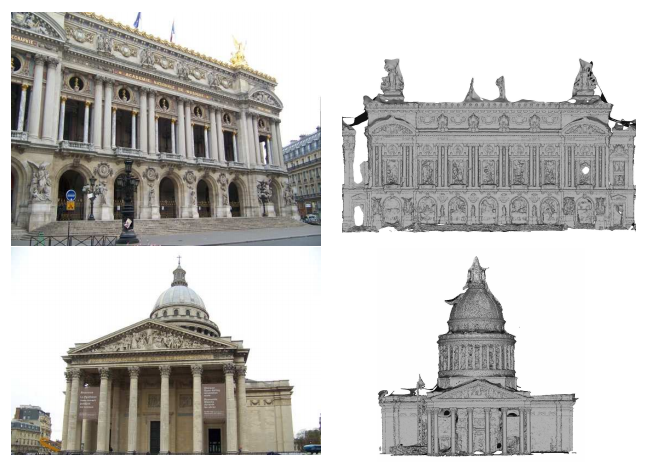
\includegraphics[width=12cm]{global-sfm}
	\caption{基于全局SfM算法的稠密重建}
	\label{global-sfm}
\end{figure}

\citet{cui2017hsfm}将两种SfM方法结合,提出了混合式SfM算法,其框架图所示。该算法首先进行图像相似部分的检测,在全局上估计相机的平均运动,然后再以增量式的方式细化每一个相机的位置,最后经过一次优化来完成地图的构建,通过实验也证明了这一算法框架在效率、准确性和鲁棒性上的优势。
\begin{figure}
	\centering
	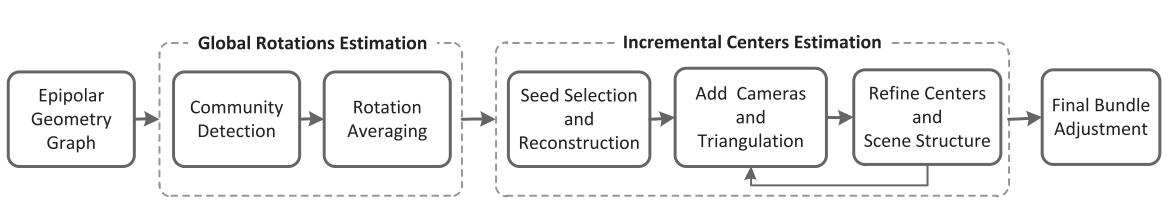
\includegraphics[width=14.5cm]{hybrid-sfm}
	\caption{混合式SfM算法流程图}
	\label{hybrid-sfm}
\end{figure}

\subsection{点云配准}
点云配准问题可以用以下数学模型来进行表述。令$X\in\mathbb{R}^{M\times 3}$和$Y\in\mathbb{R}^{N\times 3}$为分别为两个点云的坐标矩阵,其中$\boldsymbol{x}_i^T(i\in[1,M])$和$\boldsymbol{y}_j^T(j\in[1,N])$分别是矩阵$X$和$Y$中的第$i$和第$j$行,代表两个点云中第$i$和第$j$个点,假设$X$和$Y$之间有$K$个点相对应,则点云配准的目标是估计刚性变换函数$g$(可分解为旋转矩阵$R\in\mathcal{SO}(3)$和位移向量$t\in\mathbb{R}^3$),使得通过变换后两个点云能够最好地对齐:
\begin{equation}
	\label{eq: registration-function}
	\mathop{\arg\min}\limits_{R\in\mathcal{SO}(3), t\in\mathbb{R}^3} \left\| d(X,g(Y)) \right\|_2^2
\end{equation}
其中
\begin{equation}
	d(X,g(Y))=d(X,RY+t)=\sum_{k=1}^K\left\| \boldsymbol{x}_k-(R\boldsymbol{y}_k+t) \right\|_2
\end{equation}
代表$X$和变换后$Y$之间的误差。在点匹配关系已知的情况下,转移矩阵能够很好地被计算出;在转移矩阵给定的情况下点对关系也能很好的估计,但是这两个问题需要同时求解时就带来了很大的挑战\cite{huang2021comprehensive}。

点云配准领域中,最传统且最被广泛使用的莫过于ICP算法\cite{besl1992method}(Iterative Closest Point)。ICP是一种迭代式的算法,不断通过搜索最近匹配来优化旋转矩阵与平移向量,其算法可以分为以下几个步骤:
\begin{enumerate}
	\item 搜索两个点云中点到点距离最近的若干个点对;
	\item 根据搜索的点对求解两个点云之间的$\boldsymbol{R}$和$\boldsymbol{t}$;
	\item 利用计算的位姿将源点云进行变换,判断变换后两个点云的误差是否小于给定阈值;
	\item 如果误差过大,则在变换后的两个点云之间继续搜索距离最近的点对,然后重复2, 3步直至误差达到阈值或达到最大步数。
\end{enumerate}

\begin{figure}
	\centering
	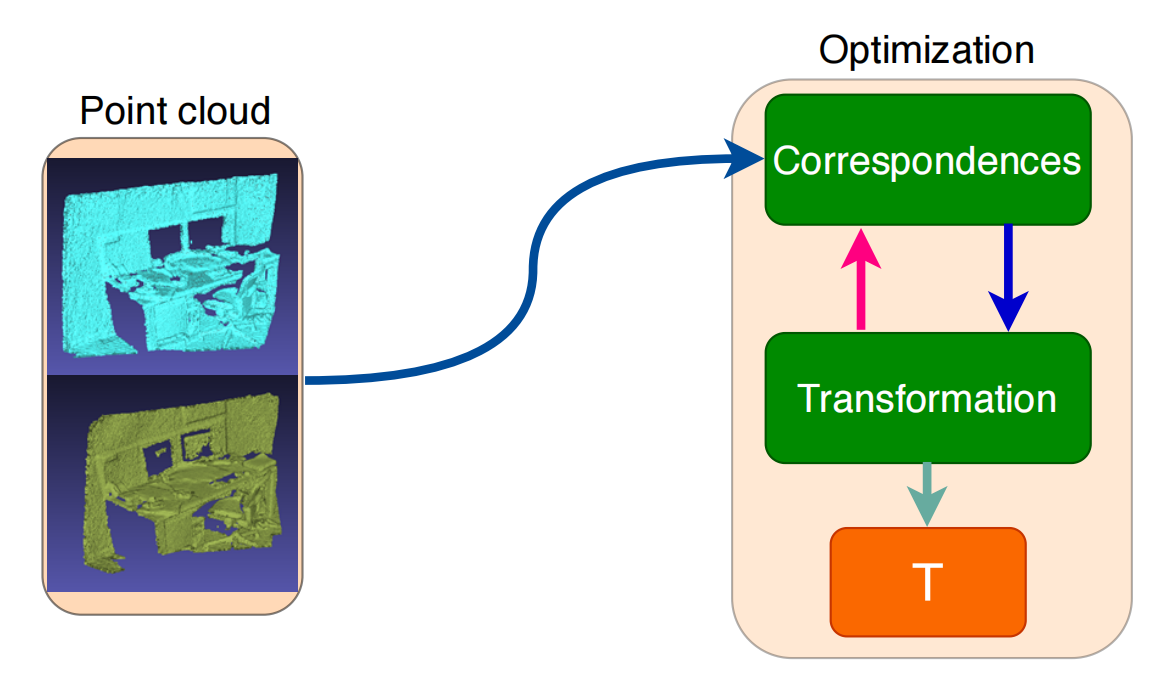
\includegraphics[width=11cm]{icp-structure}
	\caption{ICP算法流程图}
	\label{icp-structure}
\end{figure}

ICP算法根据点到点的距离关系假设了匹配对关系,然后通过迭代算法更新匹配对关系并求解转移矩阵。然而在迭代的过程中,算法不能保证收敛到全局最优,当给定的初值与真实情况相差较大时,ICP算法往往不能获得理想的结果。

在ICP算法提出之后,也有不少算法在ICP的基础上进行了改进。例如EfficientICP\cite{rusinkiewicz2001efficient}提出了几种不同的策略来提升ICP算法的速度;同时,\citet{chen1992object}将传统ICP算法中点到点距离的度量改为了点到平面距离的度量,即最小化一个点云中的点到另一个点云对应平面的垂直距离之和;沿着这个思路,\citet{forstner2017efficient}将平面到平面距离运用到了ICP算法当中,都使得ICP算法的性能得以改进。

传统的点云配准方法在过去十几年中取得了相当大的进展,但仍然在性能上存在瓶颈\cite{zhang2020deep}。在最近几年,许多基于深度学习的算法被提出,这些方法按照时间顺序如图\ref{reg-network-overview}所示,它们在Model40\cite{wu20153d}、KITTI\cite{geiger2012we}等公开数据集上获得了比传统方法更好的性能。
\begin{figure}
	\centering
	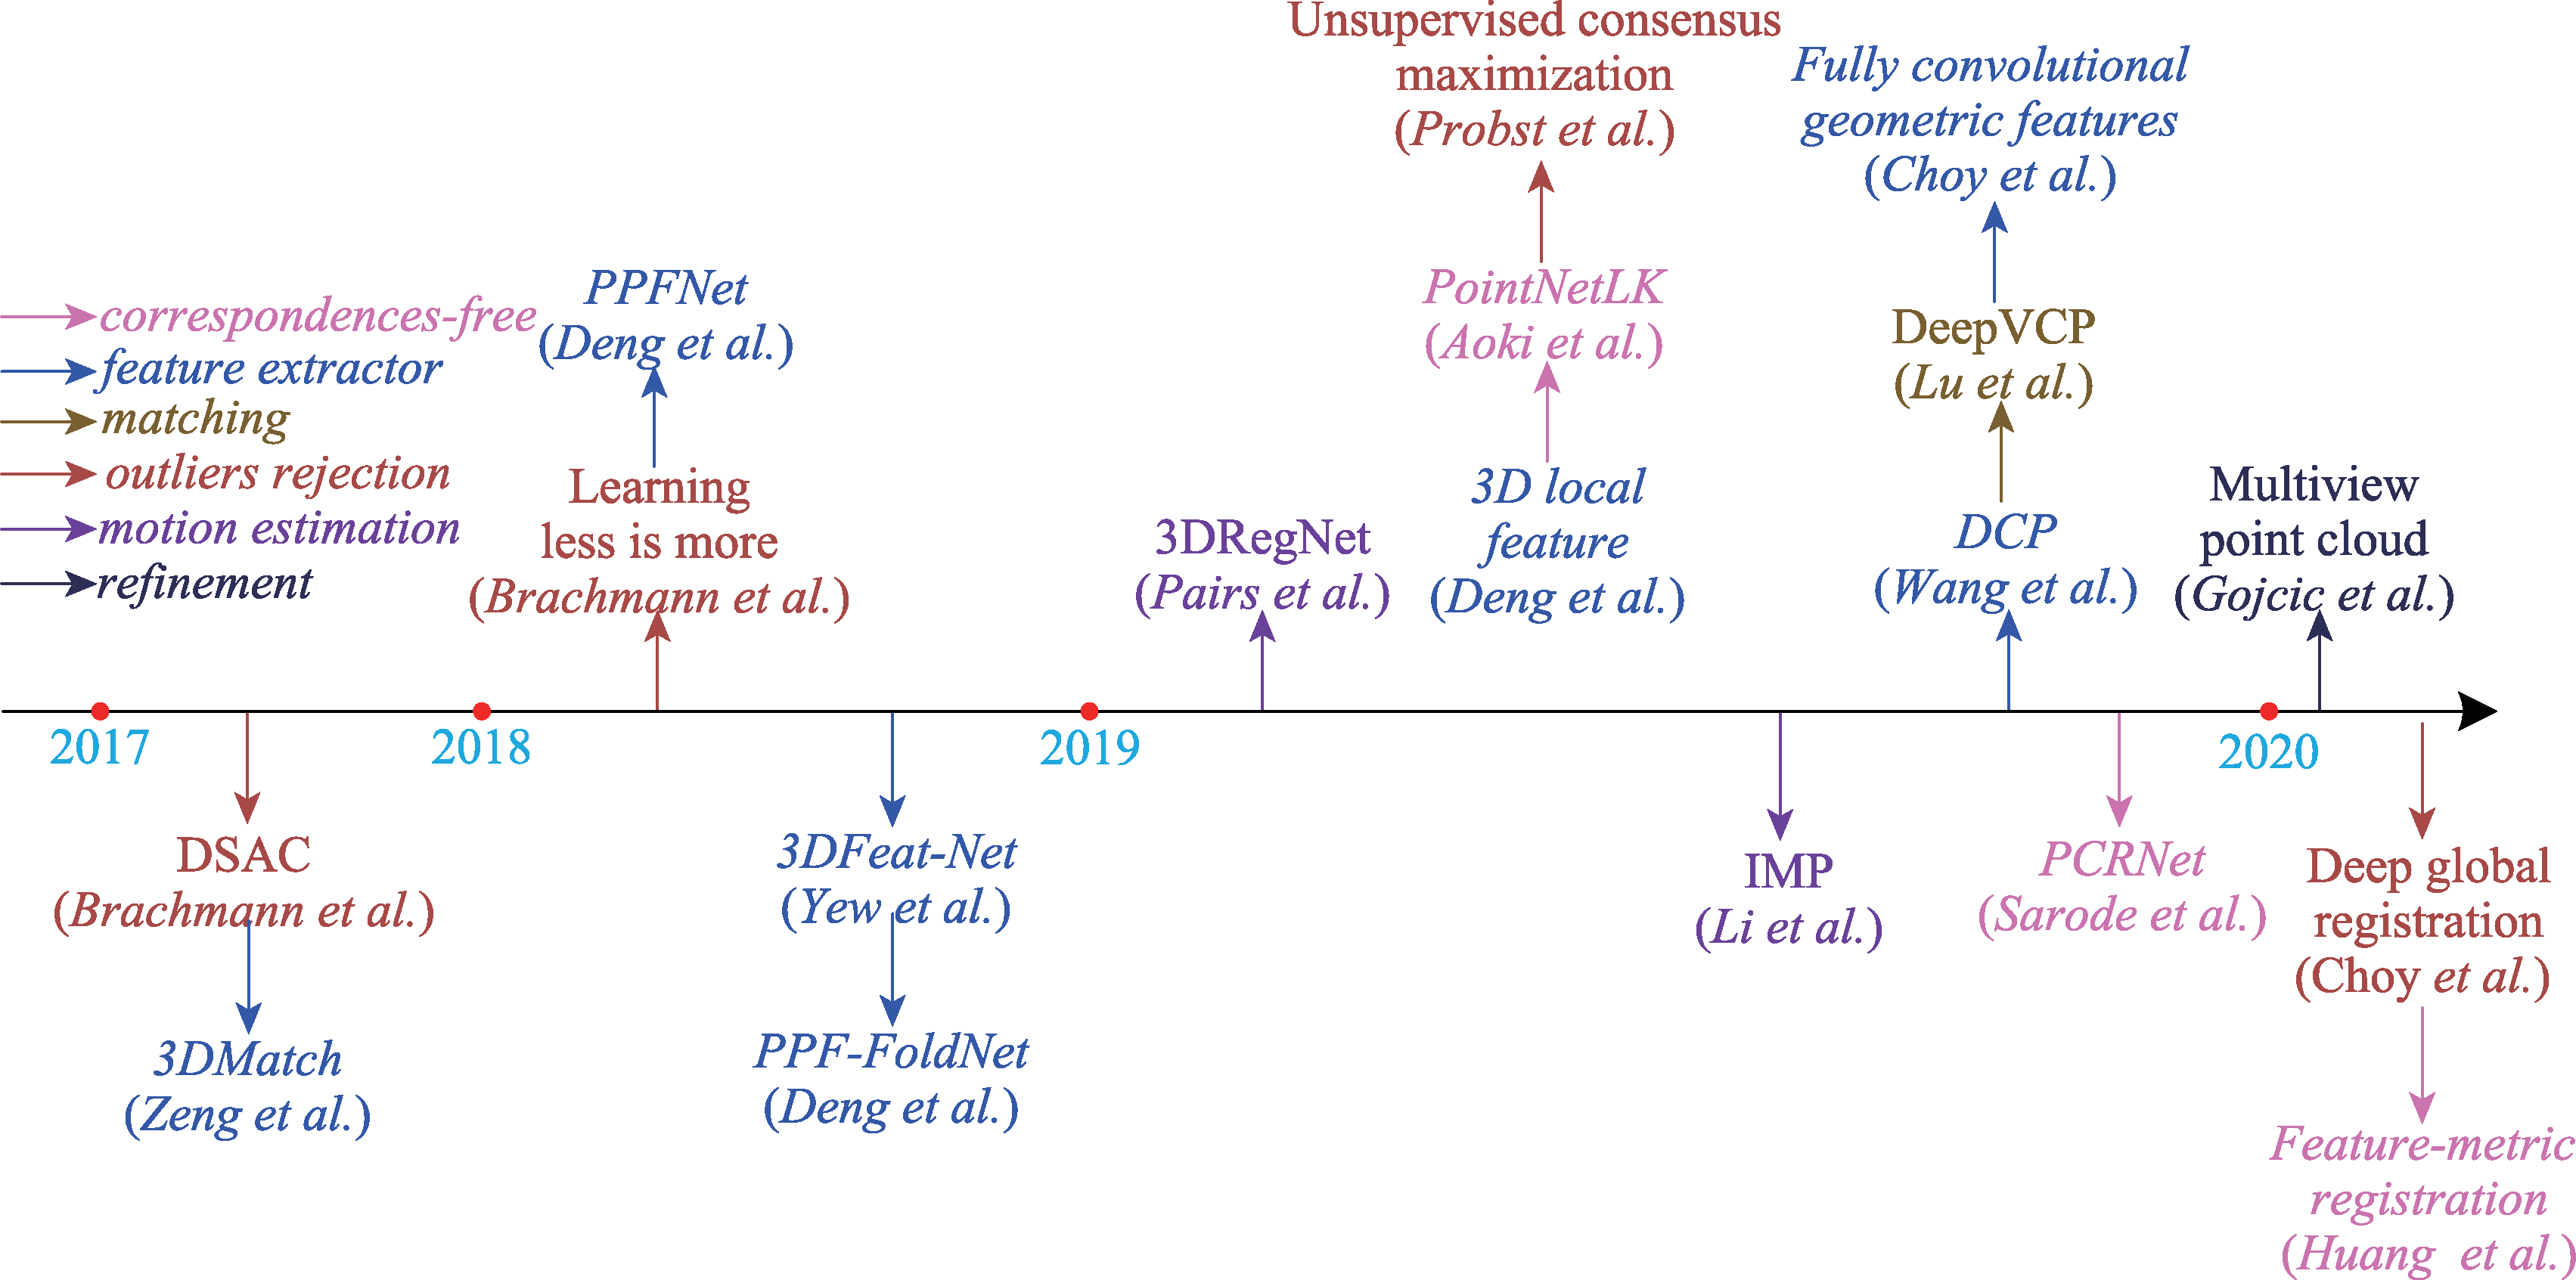
\includegraphics[width=14.5cm]{reg-network-overview}
	\caption{基于深度学习点云配准网络概述}
	\label{reg-network-overview}
\end{figure}

2017年,\citet{qi2017pointnet}提出了PointNet网络,能够用从点云中提取特征,将许多之前基于图像的任务:如分类、语义分割和目标检测等,应用到了三维点云上。2019年,PointNetLK\cite{aoki2019pointnetlk}将PointNet网络与Lucas–Kanade光流算法\cite{baker2004lucas}相结合,首次在不依赖于初始点对输入的情况下基于深度学习配准点云,从源点云与目标点云提取到的特征向量可以看做与图片特征向量相同,然后利用与图像相似的配准方法对两个点云进行配准。图\ref{pointnetlk}展示了这一网络的流程,$\phi(P_S)$和$\phi(P_T)$分别是利用PointNet从源点云和目标点云中提取到的特征,然后通过计算雅可比矩阵并利对特征进行一阶泰勒展开,来求解得到$R$和$t$,同时使用了逆向L-K算法大大提升了算法的计算效率。
\begin{figure}
	\centering
	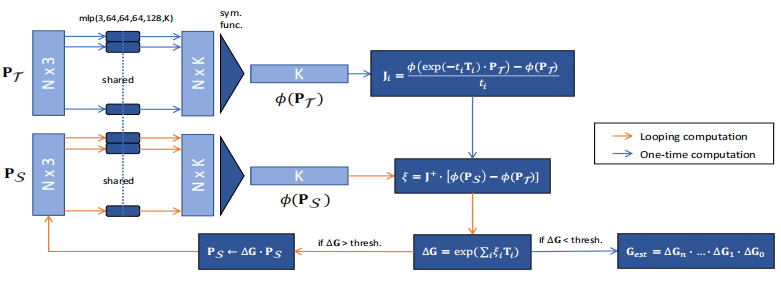
\includegraphics[width=14.5cm]{pointnetlk}
	\caption{PointNetLK网络架构}
	\label{pointnetlk}
\end{figure}

与PointNetLK类似,PCRNet\cite{sarode2019pcrnet}采用PointNet进行特征提取,其结构图图\ref{pcrnet},不同的是PCRNet在特征对齐模块中,使用了一种数据驱动的技术。首先连接两个全局特征,然后应用五个全连接层,以及输出层来直接进行位姿的估计。该算法在效率上比PointNetLK更加优秀。
\begin{figure}
	\centering
	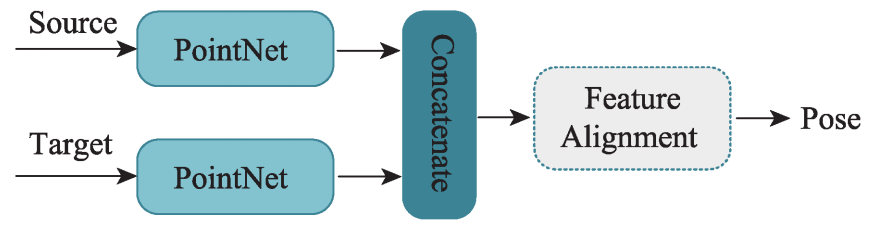
\includegraphics[width=11cm]{pcrnet}
	\caption{PCRNet网络框架}
	\label{pcrnet}
\end{figure}

在DCP网络(Deep Closest Point)\cite{wang2019deep}中,作者首次将Transformer结构\cite{vaswani2017attention}用于点云配准领域。如图\ref{dcp}所示,源点云和目标点云同样先通过一个共享参数的特征提取模块,例如PointNet,分别得到两个点云的特征,然后利用Transformer将这两者之间关联起来,得到两个点云之间的soft match矩阵,最后通过SVD分解的方式,计算得到两个点云之间的变换矩阵。
\begin{figure}
	\centering
	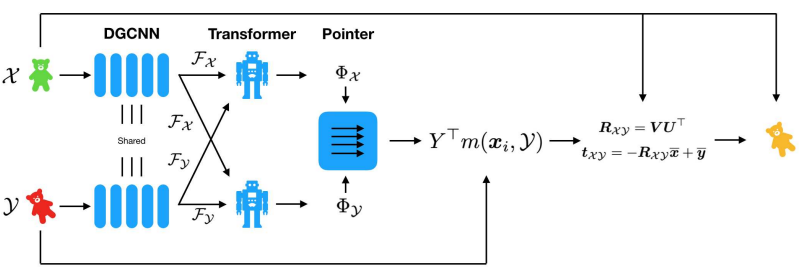
\includegraphics[width=14.7cm]{dcp}
	\caption{DCP网络框架}
	\label{dcp}
\end{figure}

总的来说,目前基于深度特征的点云配准算法性能一方面受特征提取器的影响,提取到的特征描述符越准确、对运动的灵敏度和对噪声的鲁棒性越高,则方法可能越好;另一方面对准模块决定了配准效果的上限,该模块在最终结果的生成上起着重要的作用。

\subsection{图像特征描述}
图像特征描述是指对于一张图像中感兴趣的点或图像块进行特征表述,一个好的描述符应该具有旋转不变性和尺度不变性,即空间中相同点在不同图像上的投影应该具有欧氏距离相近的特征向量,即时两张图像之间有旋转变换或者尺度变换。

为了实现尺度不变性,SIFT算法\cite{lowe2004distinctive}为输入图像构建了不同分辨率下的金字塔并对每层金字塔进行差分,在DoG空间中寻找局部极值点作为关键点\cite{lindeberg1994scale},并对关键点进行定位与梯度计算,根据梯度构建直方图并确定主方向,根据主方向保证描述符的旋转不变性,最后利用插值后的梯度直方图作为图像关键点的特征表示。

PCA-SIFT\cite{ke2004pca}在SIFT算法的基础上进行了改进,利用主成分分析(PCA)算法\cite{wold1987principal}对每个点附近像素点水平梯度和垂直梯度构成的特征向量进行降维,以此替代了SIFT算法中直接用梯度直方图的特征表示,降维的映射矩阵通过对同一类图像中的大量特征的学习而得到,这一算法能够减少描述子的维度,提升匹配的效率。

SURF算法\cite{bay2006surf}也是对SIFT的改进,它首先对求取图像的Hessian矩阵,利用Hessian矩阵挑选出图像中变化最剧烈的点作为特征点;不同于SIFT用金字塔模型来构造尺度空间,SURF对于同一大小的图像应用不同大小的盒式滤波器来进行模糊化。在特征点定位和描述子生成的方法上基本与SIFT保持一致,但是整体提取的速度更快,并且保持了旋转尺度不变性。
\begin{figure}
	\centering
	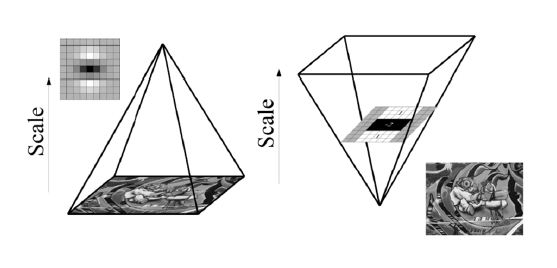
\includegraphics[width=10cm]{sift-surf}
	\caption{SIFT和SURF图像金字塔原理对比}
	\label{sift-surf}
\end{figure}

在卷积神经网络的发展和帮助下,近年来人们开始利用CNN进行特征描述学习。其中代表网络结构之一是MatchNet\cite{han2015matchnet},它的结构如图\ref{matchnet}所示,由一个深度卷积网络和一个具有三个全连接层的网络组成,前者能够从图像块(patch)中提取特征,后者用来计算提取到特征之间的相似性。MatchNet显著提高了基于手动描述符的匹配结果,显示了CNN在描述符学习方面的巨大潜力。
\begin{figure}
	\centering
	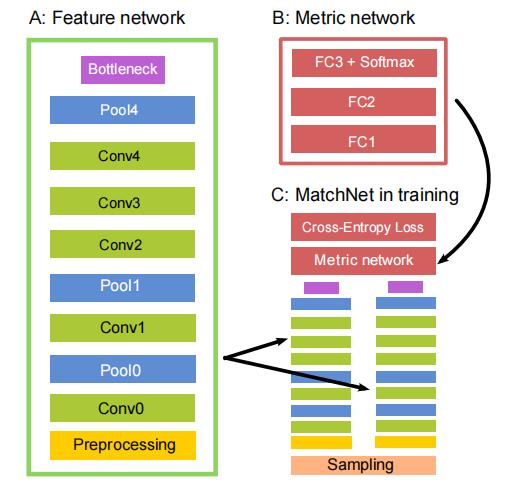
\includegraphics[width=10cm]{matchnet}
	\caption{MatchNet网络结构图}
	\label{matchnet}
\end{figure}

\subsection{视觉定位}
目前,利用视觉图像在先验激光点云中的定位问题是自动驾驶等领域的重点,这一问题的难点在于2D图像与3D点云之间的模态存在较大差异,难以构建一个统一的描述符进行特征提取与匹配。根据已有研究研究,克服这两者之间差异的方法大多是将这两者转换到同一空间中,即统一在2D空间或3D空间中完成匹配\cite{yu2020monocular}。

第一种定位方式是在2D空间中完成匹配定位。例如在前文中介绍的SLAM算法,能够通过提取特征描述子的方式完成局部的稀疏点云三维重建,并且通过图像特征来进行回环检测并减少漂移,同时还有SfM算法,也是通过2D匹配的方式完成大规模场景的三维构建。但是,图像特征对于光照条件比较敏感,在光线变化比较大的场合,难以完成鲁棒的图像匹配。\citet{wolcott2014visual}针对自动驾驶领域提出了一种新的算法,如图\ref{wolcott2014},利用先验Lidar地图,生成一些合成的针孔相机图像,并与车载实时图像利用标准化互信息(NMI)进行评估以生成定位。
\begin{figure}
	\centering
	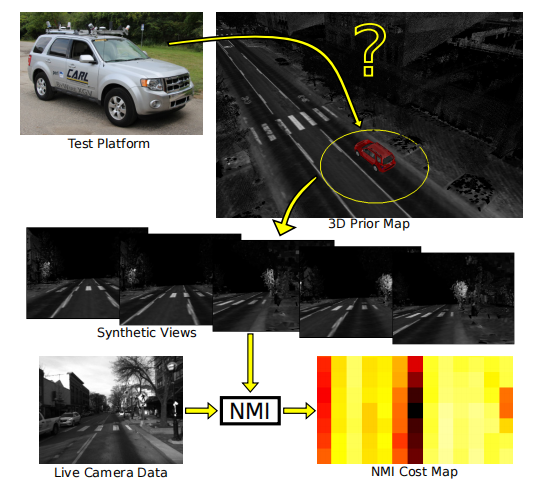
\includegraphics[width=10cm]{wolcott2014}
	\caption{基于标准化互信息的图像定位算法}
	\label{wolcott2014}
\end{figure}

第二种定位方式是在3D空间中进行匹配以计算相机位姿。如图\ref{structure-based}所示,\citet{gawel2016structure}首先通过视觉相机和IMU信息,采用SfM构建局部三维稀疏点云,然后利用三维结构描述符与稠密的离线地图进行3D-3D匹配。同时,也有学者直接利用立体相机,构建局部点云信息并匹配离线点云,然后将匹配结果耦合到VO和VIO系统中,来优化摄像机位姿\cite{kim2018stereo}。但是如上方法也存在着问题,SfM算法无法为地图提供尺度信息,因基于视觉重建的稀疏局部点云与离线地图点云之间可能无法找到对应的匹配;立体相机得到的局部点云数据量较大,因此3D匹配的耗时可能大大增强。
\begin{figure}
	\centering
	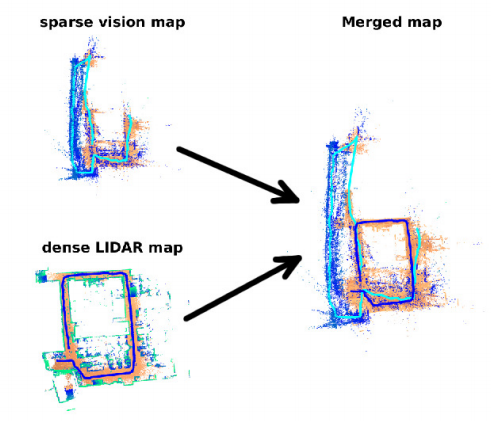
\includegraphics[width=12cm]{structure-based}
	\caption{基于3D-3D匹配的视觉定位原理图}
	\label{structure-based}
\end{figure}

\section{本文工作}
如本章第一节中介绍,目前建图与定位领域存在着许多困难与挑战,而建图与定位的精确程度又是紧密耦合的,一个高精度的地图是准确定位的基础。针对这些挑战,本文提出了一种可行且鲁棒的建图和定位的的算法流程,实现了对于大场景的离线建图与基于视觉的在线定位功能,其框架如图\ref{my-structure}所示。
\begin{figure}
	\centering
	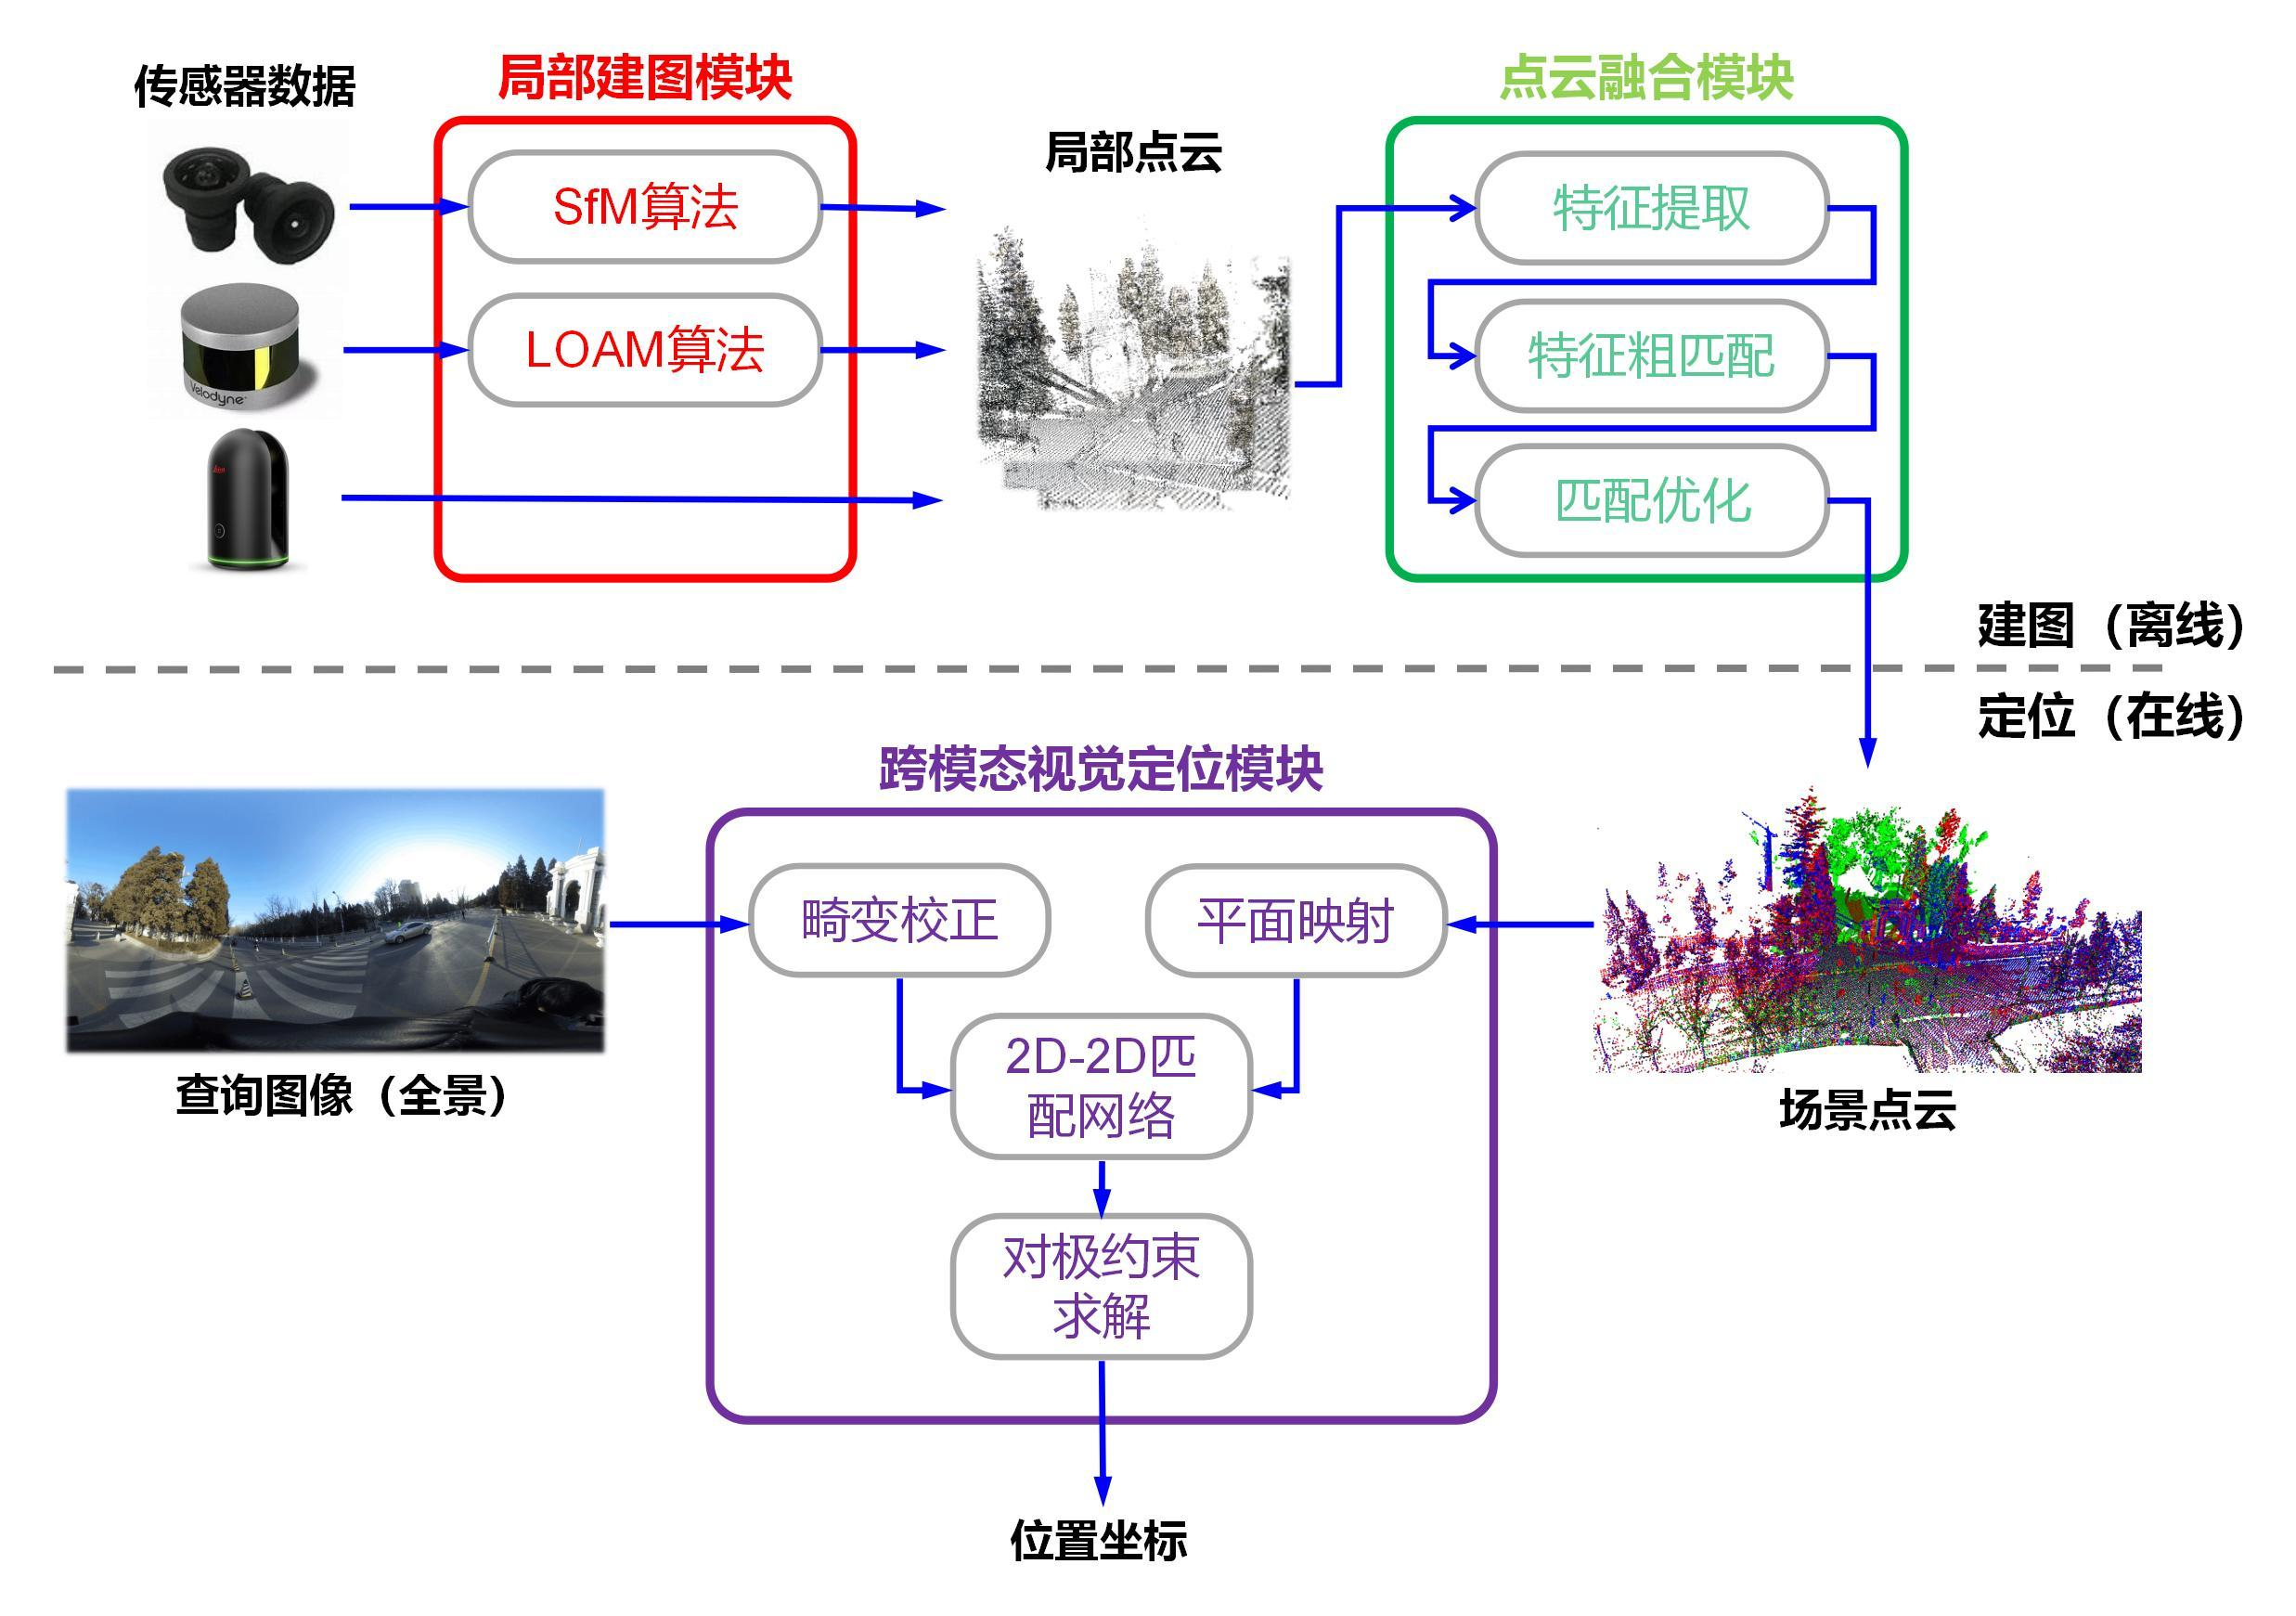
\includegraphics[width=14.5cm]{my-structure}
	\caption{本文建图-定位算法框架}
	\label{my-structure}
\end{figure}

本文算法将场景重建和定位两个部分分离开来,把复杂且计算开销大的点云匹配融合等建图相关工作放在离线部分完成,对于较为简单的图像匹配、矩阵求解等定位相关工作放在在线部分完成。

从数据采集设备来看,该算法为建图提供了不同的设备选择,既有成本低的单目相机、也有准确度较高的激光雷达与激光扫描仪,它们在数据采集与建图中各具有优劣,实际使用中可以根据需求选择合适的设备和算法;定位的设备采用了全景相机,这主要是从视野的角度出发的,因为全景相机能够无死角地将周围的所有环境图像特征融入到一张图片内,因此可以给定位提供更多的参照。

在建图环节中,本文采用了先局部后整体的方式,这主要是为了减少传统算法在大场景建图中容易出现的漂移现象,同时提升建图过程中的效率。利用SfM算法或LOAM算法,能够从单目相机或激光雷达采集到的数据中恢复场景的局部地图。若干局部地图进行两两匹配,通过一个由粗到精的匹配算法来进行融合,这一算法中结合了传统的点云特征描述子,同时也结合了深度学习对粗匹配点对进行筛选,在不依赖于初始转移估计的情况下获得了比传统ICP算法更好的效果,由此得到了全局场景的三维点云。

在定位环节中,为了避免在3D空间中耗时更大的匹配,本文选择将点云与全景图像统一到2D空间中进行匹配,根据这个思路来解决图像与激光之间的跨模态匹配问题,但这涉及到两个问题:第一,点云如何投影到图像中,并尽可能保留更多的特征;第二,全景图像带来更广阔视野的同时也会带来较大的畸变,对特征描述造成影响。针对这两个问题,本文分别设计了点云平面映射与全景畸变校正两个模块。同时,对于建图与定位环境光照条件变化的挑战,本文采用了深度学习进行描述符学习,取得了比传统特征匹配方法更鲁棒的结果。最后通过对极约束求解出查询图像在场景中的位置坐标。

\section{论文结构}
本文主要由5个章节构成,主要内容如下:
\begin{enumerate}
	\item 第\ref{ch1}章介绍了三维重建与定位技术的背景与内容,分析了此领域研究的意义与难点。同时对近年来SLAM技术和点云融合算法进行了简要介绍。
	\item 第\ref{ch2}章介绍了本文采用的局部三维重建方法,并完成了利用SfM、LOAM以及图像激光扫描仪对大礼堂场景的局部重建实验,并进行了对比。
	\item 第\ref{ch3}章介绍了本文提出的一种由粗到精的点云配准流程,能够融合局部点云生成场景全局点云地图,并分别在室内外自己采集的数据上进行了实验与分析。
	\item 第\ref{ch4}章介绍了一种视觉定位方法,能够利用先验点云地图进行绝对位置的确定,并通过实验证明了该方法的可行性。
	\item 第\ref{ch5}章对本研究的成果进行了总结,并提出了对未来可能的改进方向进行了展望。
\end{enumerate}




